\section{Aprendizaje automático}

% --------------------------------------------------------------------------------------/
% -------------------------------------------------------------------------------------/
% ------------------------------------------------------------------------------------/
\subsection*{Definiciones}
% -------------------------------------------------------------------------------------/
% ------------------------------------------------------------------------------------/
% -----------------------------------------------------------------------------------/

\subsubsection*{Definición de Microsoft \cite{MLMicros}}

El aprendizaje automático (ML) es el proceso mediante el cual se usan modelos matemáticos 
de datos para ayudar a un equipo a aprender sin instrucciones directas. Se considera 
un subconjunto de la inteligencia artificial (IA). El aprendizaje automático usa algoritmos 
para identificar patrones en los datos, y esos patrones luego se usan para crear un modelo 
de datos que puede hacer predicciones. Con más experiencia y datos, los resultados del 
aprendizaje automático son más precisos, de forma muy similar a cómo los humanos mejoran 
con más práctica.


\subsubsection*{Definición de Google \cite{MLGoogle}}

El aprendizaje automático es un subconjunto de inteligencia artificial que le permite a 
una máquina o un sistema aprender y mejorar de forma automática a partir de la experiencia. 
En lugar de una programación explícita, el aprendizaje automático usa algoritmos para 
analizar grandes cantidades de datos, aprender de las estadísticas y tomar decisiones 
fundamentadas. \\ 

Los algoritmos de aprendizaje automático mejoran el rendimiento con el paso del tiempo,
ya que se entrenan (se exponen a más datos). Los modelos de aprendizaje automático son 
el resultado o lo que el programa aprende cuando se ejecuta un algoritmo en los datos de 
entrenamiento. Cuantos más datos se usen, mejor será el modelo. 


Entonces imaginemos que vamos a entrenar a una computadora para que aprenda a reconocer gatos. 
En lugar de decirle exactamente qué es un gato, le pasamos muchas fotos de gatos y no gatos. 


\begin{center}
    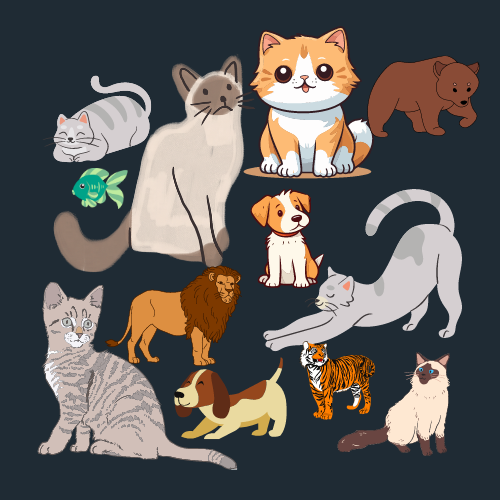
\includegraphics[scale = .5]{assets/imagenes/modulo05/step01.png}
\end{center}


La computadora va aprendiendo qué características tienen en común los gatos y cómo 
diferenciarlos de otras cosas.


\begin{center}
    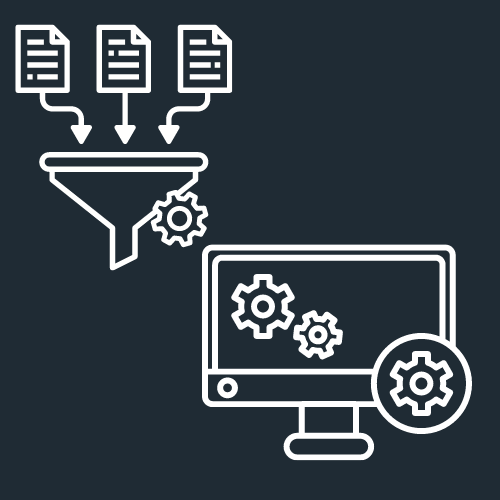
\includegraphics[scale = .5]{assets/imagenes/modulo05/step02.png}
\end{center}


Después de ver suficientes ejemplos, puede reconocer gatos en fotos nuevas.

\begin{center}
    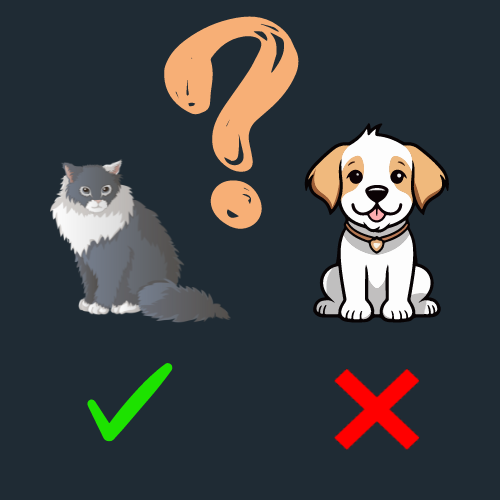
\includegraphics[scale = .5]{assets/imagenes/modulo05/step03.png}
\end{center}

Ahora el como funciona con pasos más detallados:
\begin{enumerate}
    \item Recopilar y preparar los datos: Primero, recopilamos datos de diferentes fuentes 
    y los organizamos para que la computadora pueda entenderlos. Revisamos los datos para 
    corregir errores y asegurarnos de que estén completos y consistentes.

    \item Entrenar el modelo: Dividimos los datos en dos grupos: uno para enseñar a la 
    computadora (conjunto de entrenamiento) y otro para probar lo que ha aprendido 
    (conjunto de pruebas). Usamos el conjunto de entrenamiento para enseñarle a la 
    computadora a identificar patrones y tomar decisiones.
    
    \item Validar el modelo: Después de entrenarla, probamos la computadora con el conjunto 
    de pruebas para ver si ha aprendido correctamente. Evaluamos su rendimiento y precisión 
    para asegurarnos de que pueda resolver problemas de manera confiable.
    
    \item Interpretar los resultados: Finalmente, revisamos los resultados que la computadora 
    ha dado. Analizamos la información obtenida, sacamos conclusiones y hacemos predicciones 
    basadas en lo que ha aprendido.
\end{enumerate}


% --------------------------------------------------------------------------------------/
% -------------------------------------------------------------------------------------/
% ------------------------------------------------------------------------------------/
\subsection*{Función}
% -------------------------------------------------------------------------------------/
% ------------------------------------------------------------------------------------/
% -----------------------------------------------------------------------------------/

\begin{myitemize}
    \item Reconocimiento de patrones: El aprendizaje automático puede identificar patrones en 
    datos complejos mediante el análisis de características y relaciones entre variables. 
    Por ejemplo, puede reconocer patrones en imágenes para identificar rostros humanos o detectar 
    anomalías en series temporales para prevenir fraudes financieros.

    \item Clasificación y categorización: Esta capacidad permite al aprendizaje automático clasificar 
    datos en diferentes categorías o etiquetas. Por ejemplo, puede clasificar correos electrónicos 
    como spam o no spam basándose en su contenido y características, o categorizar documentos en 
    diferentes temas según su contenido y palabras clave.
    
    \item Predicción y pronóstico: El aprendizaje automático puede predecir resultados futuros 
    utilizando modelos entrenados con datos históricos. Por ejemplo, puede predecir el rendimiento 
    de acciones en el mercado financiero, pronosticar el clima para los próximos días o anticipar 
    la demanda de productos en una tienda en línea.
    
    \item Optimización de decisiones: Ayuda a tomar decisiones más informadas y eficientes al analizar 
    grandes cantidades de datos y encontrar la mejor solución posible. Por ejemplo, puede optimizar 
    rutas de transporte para minimizar costos y tiempos de entrega, o recomendar estrategias de 
    marketing personalizadas para maximizar el retorno de inversión.
    
    \item Personalización y recomendaciones: El aprendizaje automático permite ofrecer experiencias 
    personalizadas a usuarios individuales al analizar su comportamiento y preferencias. Por ejemplo, 
    puede recomendar películas o series de televisión en plataformas de streaming basándose en el 
    historial de visualización de cada usuario, o sugerir productos relacionados en tiendas en línea 
    según las compras anteriores.
\end{myitemize}
